\documentclass[journal=jcisd8,manuscript=article]{achemso}

\SectionNumbersOn

\usepackage[version=4]{mhchem}
\usepackage[T1]{fontenc}
\usepackage{graphicx}
\usepackage{xcolor}
\usepackage{tikz}
\usetikzlibrary{arrows.meta,positioning,shapes.geometric,fit,backgrounds}

\author{Marcia Yineth Castillo}
\affiliation{Departamento de Qu\'imica, Universidad de los Andes, Bogot\'a 111711, Colombia}
\author{Gian Pietro Miscione}
\affiliation{Departamento de Qu\'imica, Universidad de los Andes, Bogot\'a 111711, Colombia}
\author{Jordi Vill\`a i Freixa}
\email{jordi.villa@uvic.cat}
\affiliation{Universitat de Vic -- Universitat Central de Catalunya, Vic, Barcelona 08500, Spain}

\title{Marcia-Automated-Workflow-for-Protein-Ligand-LIE-Linear-Interaction-Energy-Calculations: An End-to-End Q6 Application for Protein--Ligand LIE Simulations}

\abbreviations{LIE, MD, CLI, CSV}

\begin{document}

\begin{abstract}
Linear interaction energy (LIE) calculations are attractive for binding-affinity estimation because they offer a practical compromise between simulation cost and interpretability, but routine application still requires a multi-step workflow that is often assembled manually from loosely connected scripts. We present Marcia-Automated-Workflow-for-Protein-Ligand-LIE-Linear-Interaction-Energy-Calculations, an end-to-end Q6-based application workflow that integrates ligand preparation, protein--ligand complex preparation, equilibration, replicated production simulations, trajectory-quality control based on interaction-energy stability, automated extension of insufficiently converged simulations, LIE free-energy evaluation, and downstream regression analysis. The workflow is organized into repository modules for ligand-in-water and complex-in-water calculations and provides Python and shell utilities for generating Q6 input files, producing topology- and FEP-compatible systems, scanning production log files for Q-surr. electrostatic and van der Waals energy drift, flagging simulations with errors above 1 kcal/mol, and exporting ligand-wise \(\Delta G\) estimates to CSV files. A key usability feature is that stability assessment is treated as a first-class stage before free-energy reporting, reducing the risk of accepting underconverged production runs. The software is designed as an automation layer around Q6 and QLigFEP rather than as a replacement for those packages. This application note describes the architecture of the workflow, the scientific and technical advances it introduces for routine LIE studies, and the practical requirements for reproducible deployment on cluster environments.
\end{abstract}

\section{Introduction}

The linear interaction energy (LIE) method estimates ligand binding free energies from averaged electrostatic and van der Waals interaction terms obtained from end-state simulations.\cite{aqvist2001lie,gutierrez2012lie} Its appeal in drug-discovery settings comes from a favorable balance between computational cost, physical transparency, and compatibility with ligand-series studies. In practice, however, a publishable LIE study depends on more than the final equation. Users must prepare ligand and complex systems consistently, generate input files for multiple simulation stages, manage replicated molecular dynamics runs, verify that the relevant interaction energies are stable enough for analysis, and only then compute and compare \(\Delta G\) values.

Q6 provides the simulation engine needed for LIE and related free-energy calculations,\cite{bauer2018q6} while QLigFEP provides a route to ligand parameterization and related setup tasks. What is often missing is a coherent application layer that joins these capabilities into a workflow that can be followed, audited, and scaled across multiple ligands. Many groups still rely on local notes, one-off scripts, and manually edited inputs, which makes reproducibility fragile and greatly increases the effort required to extend a study from a single ligand to a series.

Marcia-Automated-Workflow-for-Protein-Ligand-LIE-Linear-Interaction-Energy-Calculations was developed to address this practical gap. The repository is organized as a complete protocol rather than a single script. It includes ligand and complex preparation modules, equilibration and production templates, analysis utilities to inspect Q-surr. interaction energies, automated generation of extended production inputs when convergence criteria are not met, LIE calculation scripts, and regression-analysis tools for reference ligands. The central contribution of the application is therefore workflow integration: it turns a scattered sequence of Q6-dependent tasks into a repeatable protocol for protein--ligand LIE calculations.

\section{Workflow Overview and Implementation}

The repository is structured around two main simulation branches, \texttt{ligands/} and \texttt{complex/}, reflecting the requirement that LIE be evaluated from separate simulations of ligand-in-water and protein--ligand complex-in-water systems. Each branch contains staged preparation and simulation logic, while the repository root provides cross-cutting analysis scripts for quality control, LIE calculation, and regression-based benchmarking.

In the ligand branch, the workflow starts from numbered ligand PDB files and generates ligand-specific library, parameter, topology, and FEP files. The documentation indicates use of QLigFEP-related tools and auxiliary scripts such as \texttt{bind\_prm.py}, \texttt{copy\_generate.py}, and \texttt{generate\_ligand\_fep.py} to produce the assets needed for Q6 execution. Equilibration inputs are generated automatically and a three-stage equilibration protocol yields restart files for production. Production input files are then created and executed as two replica-like runs per ligand.

In the complex branch, the workflow concatenates a prepared protein structure with each ligand, builds Q6 preparation inputs for the corresponding protein--ligand complex, prepares the solvated complex system, creates a one-state FEP mapping for the ligand atoms in the complex, and then runs analogous equilibration and replicated production stages. Complex-specific helper scripts include \texttt{concat\_protein\_ligands.py}, \texttt{generate\_complex.py}, \texttt{generate\_eq\_inp.sh}, and \texttt{generate\_inp\_files.py}.

Figure~\ref{fig:workflow} summarizes the full application path. After ligand and complex production runs are available, the workflow inspects Q-surr. electrostatic and van der Waals energies from the production log files. The scripts \texttt{ligand-surrounding-energies.py} and \texttt{check\_high\_errors.py} implement a simple but operationally valuable stability criterion: the trajectory is split into two halves, and the error estimate is defined as half the absolute difference between the average interaction energies of the two halves. Simulations with either electrostatic or van der Waals errors greater than 1 kcal/mol are flagged for extension. This criterion follows the practical guidance used in LIE applications.\cite{gutierrez2012lie}

If the threshold is not met, \texttt{prueba\_2.py} generates extended production input files and corresponding Slurm launch scripts under \texttt{check\_errors/}, allowing the user to continue the MD runs without rebuilding the whole system. This feature is a meaningful technical advance for day-to-day use because it turns convergence checking from a manual decision into an explicit, scripted branch of the workflow.

Once the production logs satisfy the stability requirement, \texttt{analyze\_LIE\_noqgui.py} parses ligand and complex log files through the shared \texttt{mdlog\_energies.py} module and computes the LIE estimate

\begin{multline}
\Delta G_{\mathrm{bind}} =
\beta \left[\left\langle V_{\mathrm{el}}^{\mathrm{complex,wat}} + V_{\mathrm{el}}^{\mathrm{complex,prot}}\right\rangle - \left\langle V_{\mathrm{el}}^{\mathrm{lig,wat}}\right\rangle\right] +
\alpha \left[\left\langle V_{\mathrm{vdW}}^{\mathrm{complex,wat}} + V_{\mathrm{vdW}}^{\mathrm{complex,prot}}\right\rangle - \left\langle V_{\mathrm{vdW}}^{\mathrm{lig,wat}}\right\rangle\right] +
\gamma
\end{multline}

from the extracted Q-protein and Q-water interaction terms. The root-level Slurm wrapper \texttt{analyze\_LIE\_ligands.sh} loops across ligand indices, dispatches the calculation for each ligand pair, and writes CSV summaries to \texttt{results/}. In the current repository, this launcher exposes the empirical coefficients directly in the shell script, with example values \(\alpha = 0.68\), \(\beta = 0.11\), and \(\gamma = 0.0\), making calibration choices transparent to the user.

\begin{figure}[h]
\centering
\begin{tikzpicture}[
  font=\sffamily,
  >=Latex,
  box/.style={
    rounded corners=3pt,
    draw=#1,
    fill=#1!8,
    line width=0.9pt,
    minimum width=3.1cm,
    minimum height=1.2cm,
    align=center
  },
  decision/.style={
    diamond,
    aspect=2.0,
    draw=#1,
    fill=#1!8,
    line width=0.9pt,
    inner xsep=1.2ex,
    inner ysep=1.0ex,
    align=center
  },
  arrow/.style={-{Latex[length=3mm]}, line width=0.9pt, draw=black!70},
  note/.style={font=\small\itshape, align=center}
]

\definecolor{navy}{RGB}{30,65,110}
\definecolor{teal}{RGB}{53,137,132}
\definecolor{orange}{RGB}{214,132,61}
\definecolor{crimson}{RGB}{160,63,73}

\node[box=navy] (start) at (0,0) {Prepared protein, ligand,\\and Q6 parameter inputs};
\node[box=teal, minimum width=4.2cm, minimum height=1.5cm] (lig) at (-4.6,-2.4) {Ligand-in-water\\prep, equilibration, production\\\(\langle V_{\mathrm{el}}^{\mathrm{lig,wat}}\rangle,\ \langle V_{\mathrm{vdW}}^{\mathrm{lig,wat}}\rangle\)};
\node[box=teal, minimum width=4.6cm, minimum height=1.5cm] (comp) at (4.6,-2.4) {Protein--ligand complex\\prep, equilibration, production\\\(\langle V_{\mathrm{el}}^{\mathrm{comp}}\rangle,\ \langle V_{\mathrm{vdW}}^{\mathrm{comp}}\rangle\)};
\node[box=orange, minimum width=4.6cm, minimum height=1.5cm] (logs) at (0,-5.2) {Q-surr.\ energy extraction\\from production log files};
\node[decision=crimson] (qc) at (0,-7.9) {\(\varepsilon = \tfrac{1}{2}\lvert \bar{V}_1 - \bar{V}_2 \rvert\)\\[1pt]
\(< 1\ \mathrm{kcal\,mol^{-1}}\)?};
\node[box=crimson, minimum width=5.3cm, minimum height=1.9cm] (calc) at (0,-10.9) {LIE calculation and analysis\\\(\Delta G_{\mathrm{bind}} = \beta\,\Delta\langle V_{\mathrm{el}}\rangle + \alpha\,\Delta\langle V_{\mathrm{vdW}}\rangle + \gamma\)\\CSV summaries + regression plots};

\draw[arrow] (start) -- (lig);
\draw[arrow] (start) -- (comp);
\draw[arrow] (lig) -- (logs);
\draw[arrow] (comp) -- (logs);
\draw[arrow] (logs) -- (qc);
\draw[arrow] (qc) -- (calc);

\node[note] at (-4.6,-3.8) {Ligand-in-water interaction\\averages used as the reference state};
\node[note] at (4.6,-3.8) {Complex-state interaction averages\\from ligand--protein and ligand--water terms};
\node[note] at (0,-6.3) {Plots and reports identify\\unstable trajectories};
\node[note] at (0,-9.3) {If the threshold fails, extension inputs are\\written under \texttt{check\_errors/}};

\end{tikzpicture}

\caption{General scheme of the Marcia-Automated-Workflow-for-Protein-Ligand-LIE-Linear-Interaction-Energy-Calculations application. The workflow prepares ligand and complex systems separately, runs replicated Q6 equilibration and production simulations, checks Q-surr. interaction-energy stability, branches to MD extension when the error threshold is not met, and finally computes LIE binding free energies and downstream analyses.}
\label{fig:workflow}
\end{figure}

The repository also includes downstream evaluation utilities such as \texttt{DG\_regression\_reference\_ligands.py}, which fits a linear regression between experimental and calculated free energies and reports metrics including \(R^2\), MAE, and RMSE. This places the workflow beyond mere simulation setup by supplying an explicit postprocessing path for reference-ligand validation.

\section{Usability Advances}

The principal advance of this application is that it formalizes the entire LIE protocol, not only the final energy calculation. The repository provides explicit module boundaries for ligand preparation, complex preparation, equilibration, production, quality control, free-energy estimation, and regression analysis. This reduces hidden know-how and makes the protocol easier to hand off between users.

The second major advance is the integration of quality control into the default workflow. Many practical LIE pipelines compute \(\Delta G\) directly from whatever production trajectory is available. Here, the scripts explicitly inspect Q-surr. interaction energies, generate per-log plots, identify simulations that exceed an error threshold, and support extension of the simulation length before free-energy reporting. This is a scientifically important usability feature because it encourages users to reject unstable trajectories rather than accept them silently.

Third, the workflow is cluster-oriented and scriptable. Slurm launchers are supplied for preparation, production, extension, and LIE evaluation, which makes the application suitable for routine academic HPC use. The output is machine-readable, primarily as CSV tables and report files, so the calculated energies can be integrated directly into later benchmarking or medicinal-chemistry analysis steps.

Finally, the software exposes empirical choices instead of burying them. Simulation lengths, coefficient values, and directory expectations are visible in the scripts and tutorials, which makes the protocol easier to audit and adapt. For a JCIM Application Note, this combination of automation, traceability, and reviewer-testable behavior is more important than claiming methodological novelty.

\section{Demonstration Case in the Current Repository}

The target repository already contains a worked example spanning ligand and complex setup files, production logs, quality-control plots, an error report, and at least one LIE result CSV file. It also contains a reference-ligand regression plot for an MDM2 inhibitor series. This is a stronger basis for an application note than the previously used analysis-only repository because it shows the end-to-end protocol in a single codebase.

For the final journal submission, the demonstration should be framed as an end-to-end MDM2 inhibitor workflow: start from a prepared protein and ligand structures, generate the ligand and complex Q6 systems, run equilibration and replicated production, inspect the Q-surr. interaction-energy stability, extend simulations if needed, compute ligand-wise LIE \(\Delta G\) values, and compare selected reference ligands against experiment. The current repository contents already support that narrative and provide concrete filenames and outputs that reviewers can inspect.

\section{Data and Software Availability}

The software described here should be made available through a public versioned repository under the name used in the manuscript title, together with a tagged release archived through a persistent repository service. The release should include the ligand and complex tutorials, the helper scripts required for input generation and analysis, representative example files, and a reviewer-accessible minimal test case. Because the workflow depends on Q6 and QLigFEP, those dependencies should be cited and linked separately.\cite{bauer2018q6,q6repo,qligfeprepo}

The current implementation assumes an HPC-style environment with Python 3.8 and Slurm available for execution of the supplied batch scripts. Some preparation steps also rely on external software in the ligand module. The final manuscript should state clearly which components are operating-system agnostic and which are expected to run in a Linux cluster setting. That distinction is important for compliance with JCIM software-availability expectations.

\section{Associated Content}

\textbf{Supporting Information.} Suggested Supporting Information for the final submission includes a reviewer test protocol, a minimal end-to-end example for one ligand, the directory schema expected by the analysis scripts, and a compact table mapping each workflow stage to its inputs and outputs.

\section{Author Information}

\textbf{Corresponding Author}

Jordi Vill\`a i Freixa, Universitat de Vic -- Universitat Central de Catalunya, Vic, Barcelona 08500, Spain; Email: jordi.villa@uvic.cat

\textbf{Notes}

The authors declare no competing financial interest.

\section{Acknowledgments}

This draft reserves space for funding, institutional computing resources, and any acknowledgments related to Q6, QLigFEP, and the preparation of the MDM2 ligand series used as the demonstration case.

\bibliography{refs}

\begin{tocentry}
\centering
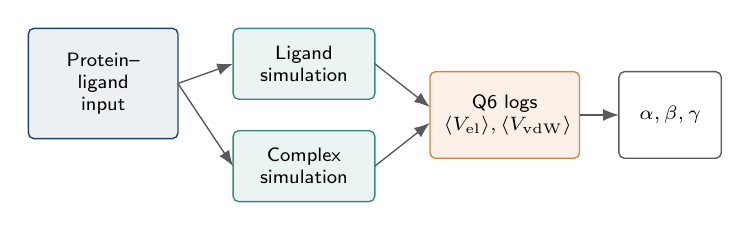
\begin{tikzpicture}[font=\sffamily\fontsize{7.2}{8}\selectfont]
  \definecolor{navy}{RGB}{30,65,110}
  \definecolor{teal}{RGB}{53,137,132}
  \definecolor{orange}{RGB}{214,132,61}
  \definecolor{grayline}{RGB}{90,90,90}

  \draw[rounded corners=2pt, fill=navy!8, draw=navy, line width=0.5pt] (0.0,1.6) rectangle (1.9,3.0);
  \node[align=center,text width=1.5cm] at (0.95,2.3) {Protein--ligand\\input};

  \draw[rounded corners=2pt, fill=teal!10, draw=teal, line width=0.5pt] (2.6,2.1) rectangle (4.4,3.0);
  \node[align=center,text width=1.4cm] at (3.5,2.55) {Ligand\\simulation};

  \draw[rounded corners=2pt, fill=teal!10, draw=teal, line width=0.5pt] (2.6,0.8) rectangle (4.4,1.7);
  \node[align=center,text width=1.4cm] at (3.5,1.25) {Complex\\simulation};

  \draw[-{Latex[length=2mm]}, line width=0.5pt, color=grayline] (1.9,2.3) -- (2.6,2.55);
  \draw[-{Latex[length=2mm]}, line width=0.5pt, color=grayline] (1.9,2.3) -- (2.6,1.25);

  \draw[rounded corners=2pt, fill=orange!12, draw=orange, line width=0.5pt] (5.1,1.35) rectangle (7.0,2.45);
  \node[align=center,text width=1.55cm] at (6.05,1.90) {Q6 logs\\\(\langle V_{\mathrm{el}}\rangle,\langle V_{\mathrm{vdW}}\rangle\)};
  \draw[-{Latex[length=2mm]}, line width=0.5pt, color=grayline] (4.4,2.55) -- (5.1,2.0);
  \draw[-{Latex[length=2mm]}, line width=0.5pt, color=grayline] (4.4,1.25) -- (5.1,1.8);

  \draw[rounded corners=2pt, fill=white, draw=grayline, line width=0.5pt] (7.5,1.35) rectangle (8.8,2.45);
  \node[align=center,text width=1.0cm] at (8.15,1.90) {\(\alpha,\beta,\gamma\)};
  \draw[-{Latex[length=2mm]}, line width=0.5pt, color=grayline] (7.0,1.90) -- (7.5,1.90);
\end{tikzpicture}
\end{tocentry}

\end{document}
